\chapter{More results from usecase chapter}
\label{app:noise_analysis}

\section{PaTAS Confidence Signal: Per-Sample Input Trust Feedforward}
\label{sec:per_sample}
This section presents a complementary experiment to \Cref{sec:patas_discriminator}, 
in which the trust feedforward uses per-sample calibrated input trust rather 
than a fully trusted opinion. In the main experiment, the feedforward receives 
a fully trusted input opinion $(1, 0, 0)$ for all samples regardless of their 
actual noise level, isolating the contribution of parameter trust accumulated 
during training. Here, each test sample $i$ instead receives its own calibrated 
input trust opinion $T_{x_i} = \text{feature\_trust}(\sigma_i)$, where $\sigma_i$ 
is the actual noise level drawn for that sample, so that both input quality 
and parameter trust contribute jointly to the output opinion.

\Cref{fig:patas_persample} visualizes the resulting opinion masses and 
discriminative gaps.

\begin{figure}[p]
\centering
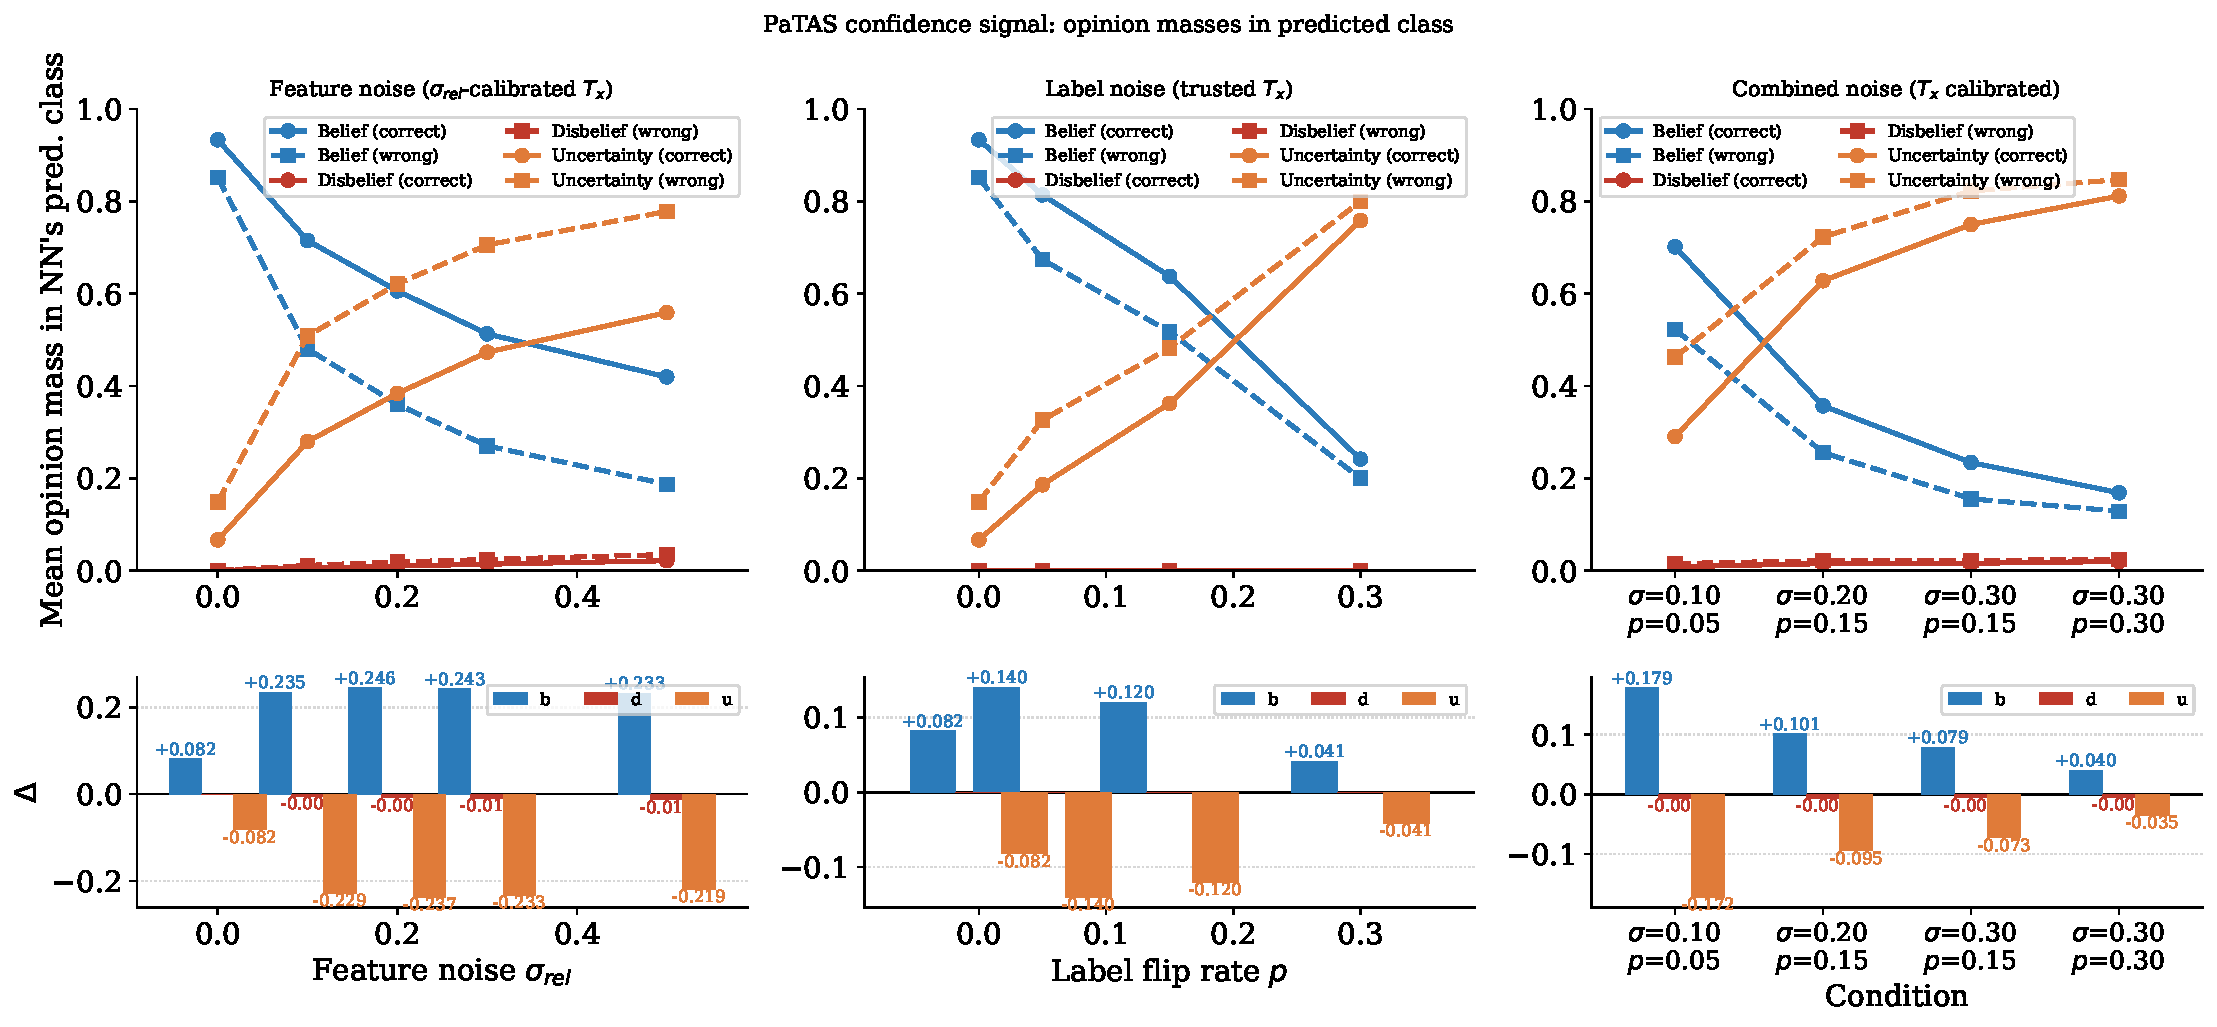
\includegraphics[width=\textwidth]{img/usecase/patas_effectiveness_agg_per_sample.pdf}
\caption{\ac{PaTAS} opinion masses with per-sample calibrated input trust 
feedforward. Top: mean opinion values for correctly-classified (solid lines, 
circles) versus misclassified (dashed lines, squares) samples. Bottom: 
$\Delta = \text{correct} - \text{wrong}$, showing the discriminative gap 
per component. Left: feature noise. Center: label noise. Right: combined 
noise.}
\label{fig:patas_persample}
\end{figure}

Three observations distinguish this experiment from the main results of 
\Cref{sec:patas_discriminator}.

\paragraph{Disbelief is no longer zero under feature noise.}
When per-sample input trust is fed forward, disbelief becomes a small but 
non-negligible component of the discriminative signal under feature noise: 
$\Delta d$ ranges from $-0.006$ at $\sigma_{\text{rel}} = 0.10$ to $-0.013$ 
at $\sigma_{\text{rel}} = 0.50$. This is consistent with the trust 
quantification design: the feature trust opinion assigns a small disbelief 
component $d = \sigma_{\text{rel}}(1 - u)$ to each sample, and this 
propagates through the \ac{TNN} to produce a non-zero disbelief in the 
output opinion. The effect is small relative to the belief and uncertainty 
gaps, but it confirms that the disbelief channel carries meaningful 
provenance information when input quality is explicitly encoded.

\paragraph{The discriminative gap $\Delta b$ is larger than in the 
fully-trusted case.}
Under feature noise, $\Delta b$ ranges from $+0.235$ at 
$\sigma_{\text{rel}} = 0.10$ to $+0.243$ at $\sigma_{\text{rel}} = 0.20$, 
slightly higher than the corresponding values of $+0.228$ and $+0.237$ in 
the main experiment. This reflects the additional discriminative power 
contributed by the per-sample input trust: samples with lower noise receive 
higher input belief, which amplifies the output belief gap between correct 
and incorrect predictions. Under label noise the values are identical to 
the main experiment, as expected: the label noise experiment uses fully 
trusted feature inputs in both settings.

\paragraph{The combined noise results show non-zero disbelief gaps.}
Under combined noise, $\Delta d$ is small but consistently negative 
(ranging from $-0.005$ to $-0.007$), confirming that when both feature 
and label corruption are present and input trust is calibrated per sample, 
the disbelief channel contributes a weak additional discriminative signal 
beyond what belief and uncertainty alone provide.

Together, these results confirm that per-sample input trust feedforward 
produces a richer and marginally more discriminative trust signal than the 
fully-trusted baseline, at the cost of requiring knowledge of the per-sample 
noise level $\sigma_i$ at test time. In deployment settings where this 
information is available (for instance, from sensor quality metadata), 
the per-sample variant is preferred. Where it is not, the fully-trusted 
feedforward of \Cref{sec:patas_discriminator} provides a conservative 
but still informative trust signal.


\section{Extended Coverage--Accuracy and ROC Analysis for Selective Prediction}
\label{app:coverage_roc}
 
\Cref{sec:selective_prediction} summarizes the coverage--accuracy
trade-off between \ac{PaTAS} and softmax filtering at representative
operating points (e.g., accuracy at 20\% coverage). This appendix
presents the complete curves for all four panels of each noise axis,
together with the corresponding ROC curve and AUC for each condition,
obtained by treating the filtering score (\ac{PaTAS} projected
probability $\pi = b + u/2$, or the softmax maximum probability) as a
ranking signal and correctness of the \ac{NN}'s prediction as the
binary outcome.
 
\subsection{Feature Noise}
\label{app:coverage_roc_feature}
 
\begin{figure}[h]
\centering
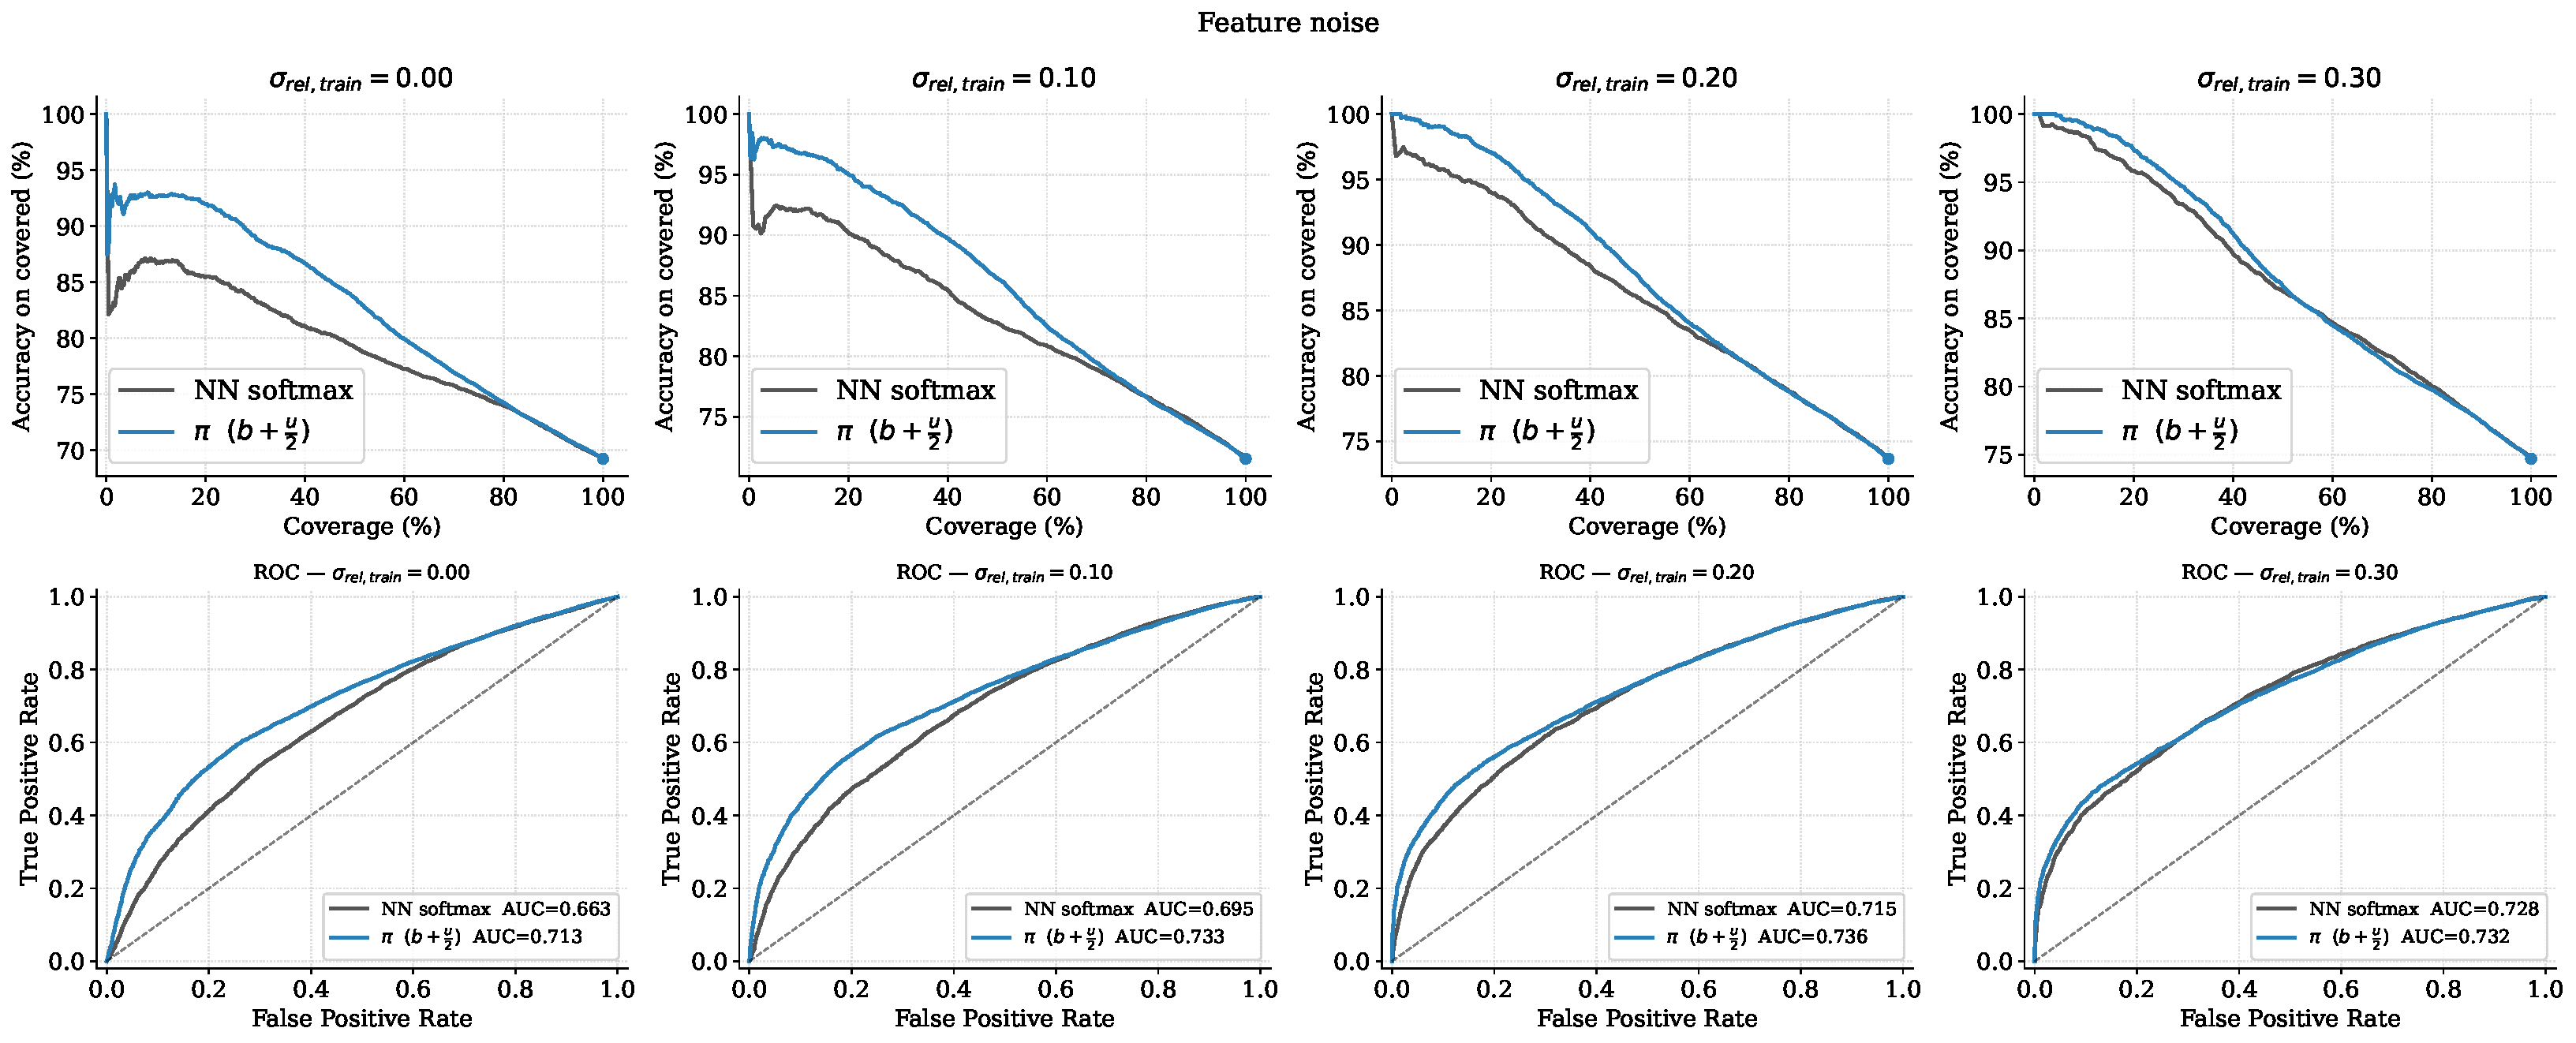
\includegraphics[width=\linewidth]{img/usecase/app/coverage_accuracy_feature.pdf}
\caption{Top: coverage--accuracy curves under feature noise, extending
\Cref{fig:coverage_accuracy_feature}, for
$\sigma_{\text{rel,train}} \in \{0.00, 0.10, 0.20, 0.30\}$ with test
noise $\sigma_{\text{rel,test}} \sim \text{Uniform}(0,1)$. Bottom:
corresponding ROC curves and AUC for \ac{PaTAS} ($\pi = b + u/2$)
versus softmax maximum probability.}
\label{fig:app_coverage_roc_feature}
\end{figure}
 
\Cref{fig:app_coverage_roc_feature} confirms the coverage--accuracy
advantage reported in \Cref{sec:selective_prediction} at the level of
overall ranking quality. \ac{PaTAS} attains a higher AUC than softmax
at every training noise level: $0.713$ versus $0.663$ at
$\sigma_{\text{rel,train}} = 0.00$, $0.733$ versus $0.695$ at
$\sigma_{\text{rel,train}} = 0.10$, and $0.736$ versus $0.715$ at
$\sigma_{\text{rel,train}} = 0.20$. The gap narrows as training noise
increases, reaching near-parity at $\sigma_{\text{rel,train}} = 0.30$
($0.732$ versus $0.728$), consistent with the convergence of the two
coverage--accuracy curves at higher training noise discussed in
\Cref{sec:selective_prediction} and with the regularization effect of
input noise during training.
 
\subsection{Label Flipping}
\label{app:coverage_roc_label}
 
\begin{figure}[h]
\centering
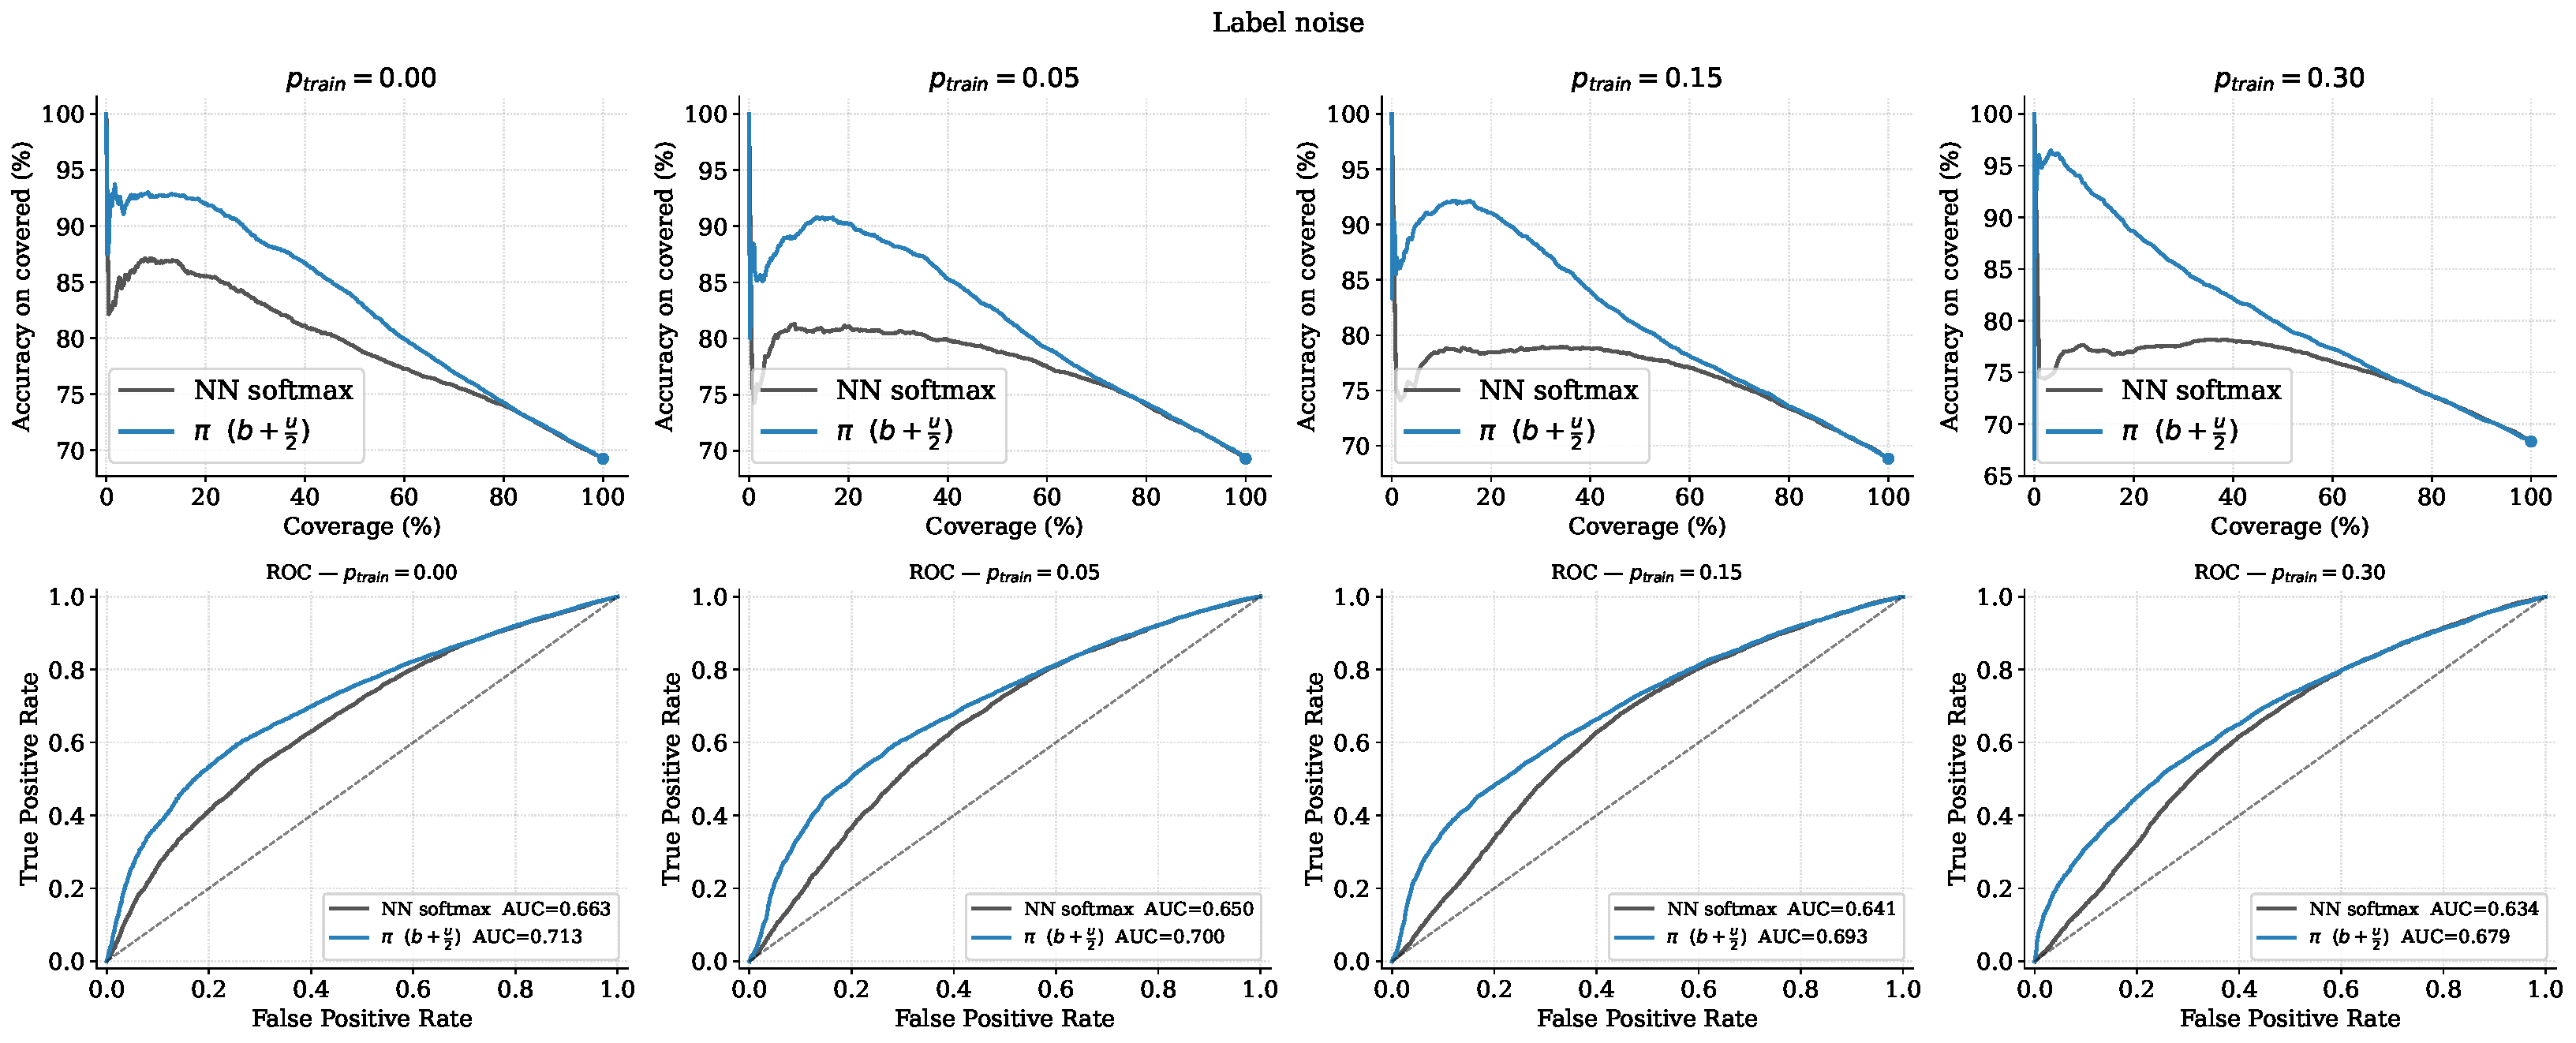
\includegraphics[width=\linewidth]{img/usecase/app/coverage_accuracy_label.pdf}
\caption{Top: coverage--accuracy curves under label flipping, extending
\Cref{fig:coverage_accuracy_label}, for
$p_{\text{train}} \in \{0.00, 0.05, 0.15, 0.30\}$. Bottom: corresponding
ROC curves and AUC for \ac{PaTAS} versus softmax.}
\label{fig:app_coverage_roc_label}
\end{figure}
 
Under label flipping, the AUC advantage of \ac{PaTAS} over softmax is
essentially constant across the evaluated flip rates: $+0.050$ at
$p_{\text{train}} = 0.00$ ($0.713$ vs.\ $0.663$), $+0.050$ at
$p_{\text{train}} = 0.05$ ($0.700$ vs.\ $0.650$), $+0.052$ at
$p_{\text{train}} = 0.15$ ($0.693$ vs.\ $0.641$), and $+0.045$ at
$p_{\text{train}} = 0.30$ ($0.679$ vs.\ $0.634$). Unlike the
feature-noise case, the gap does not narrow with increasing corruption,
mirroring the sustained advantage observed in the coverage--accuracy
curves of \Cref{sec:selective_prediction} and reinforcing the
conclusion that \ac{PaTAS} retains discriminative power under label
corruption even as the absolute AUC of both filters declines.
 
\subsection{Combined Noise}
\label{app:coverage_roc_combined}
 
\begin{figure}[h]
\centering
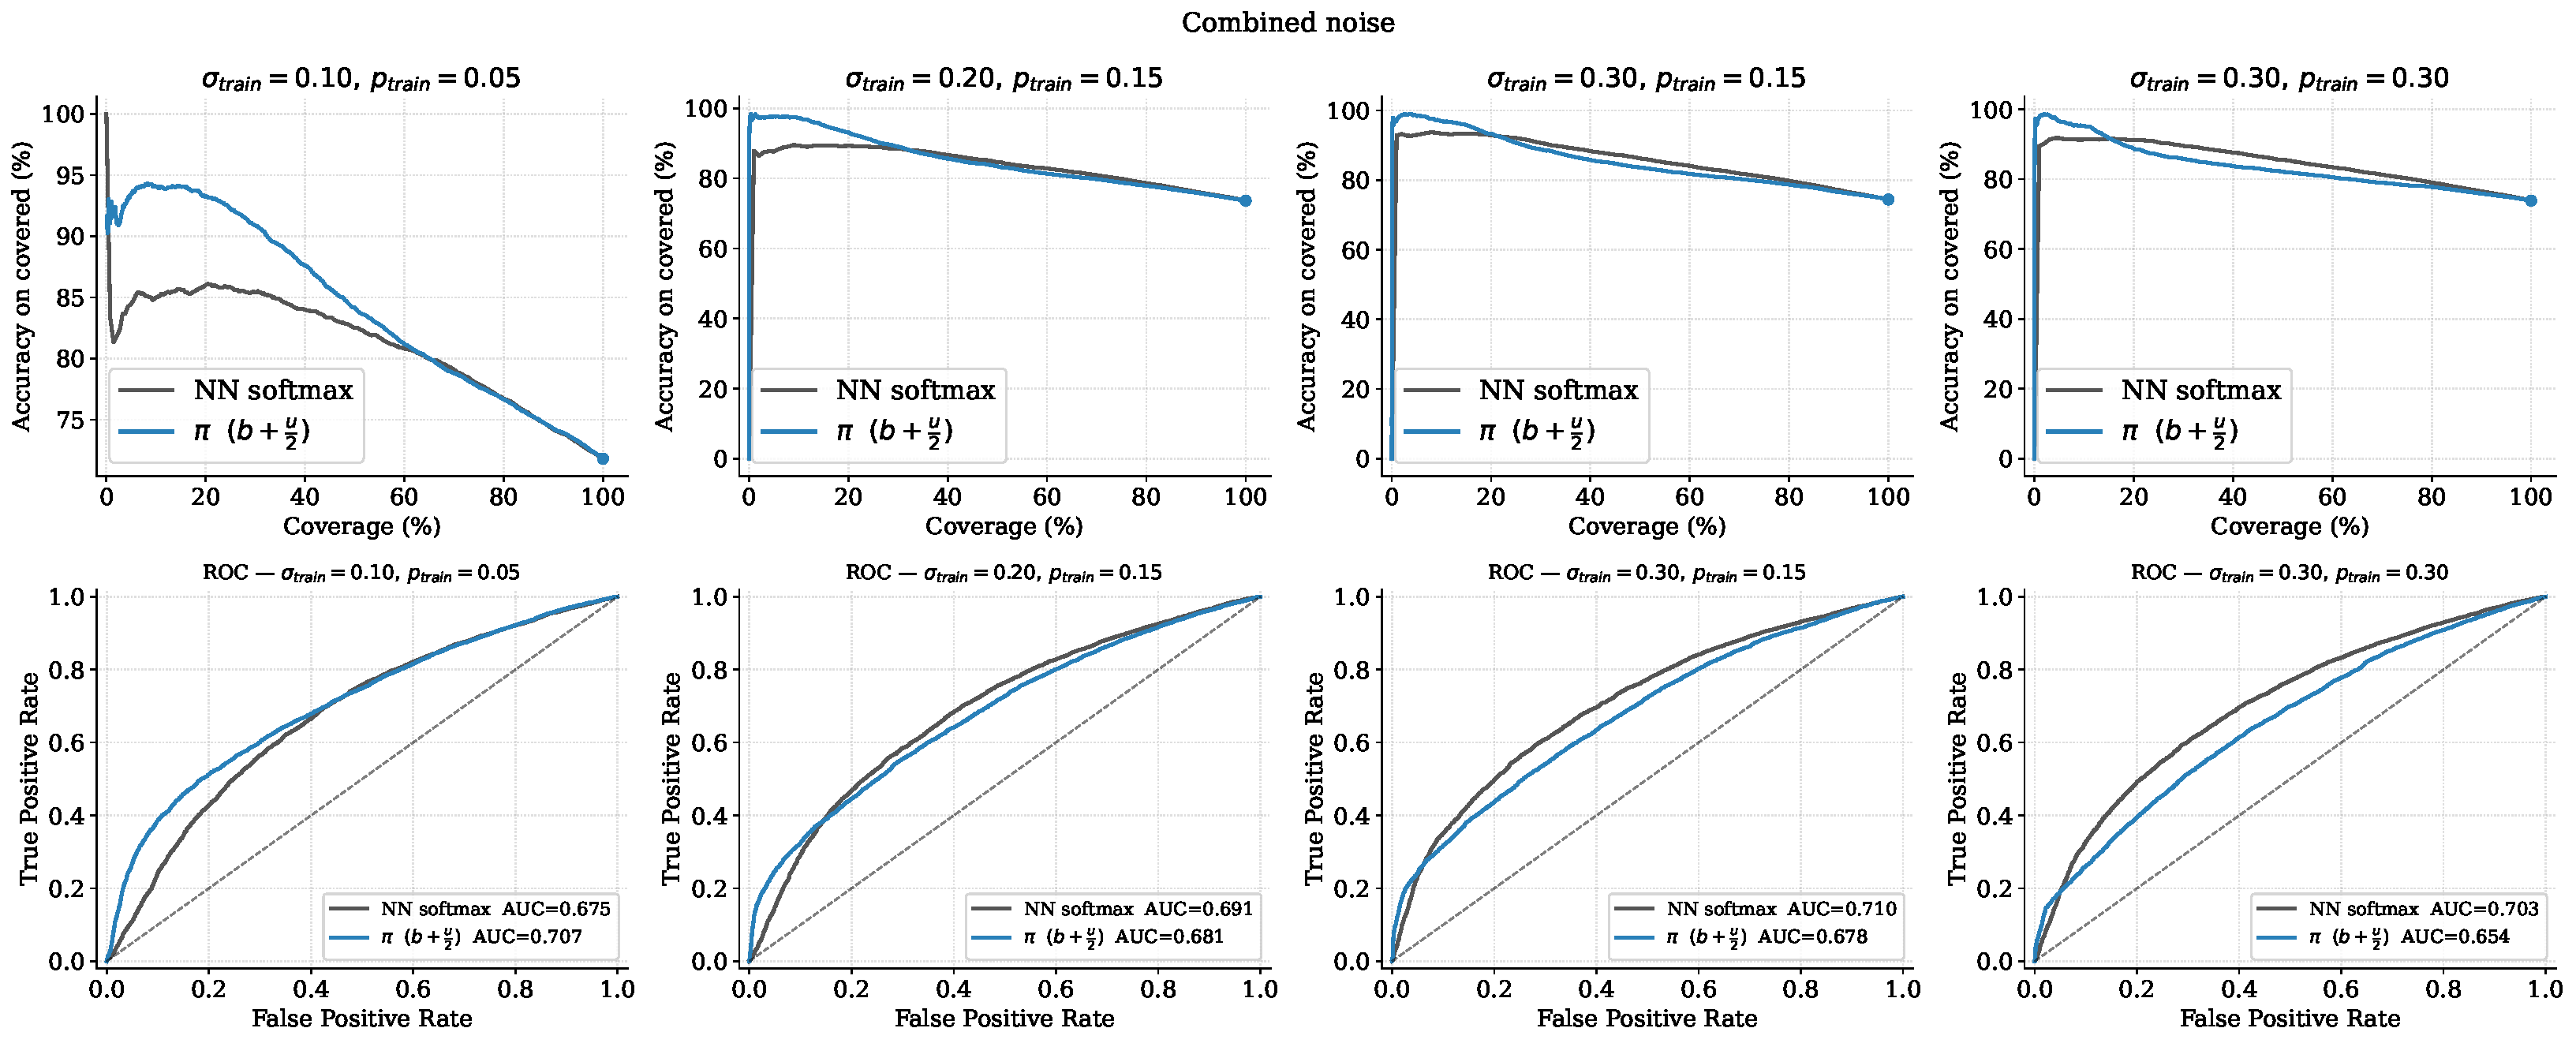
\includegraphics[width=\linewidth]{img/usecase/app/coverage_accuracy_combined.pdf}
\caption{Top: coverage--accuracy curves under combined feature and label
noise, extending \Cref{fig:coverage_accuracy_combined}, for
$(\sigma_{\text{train}}, p_{\text{train}}) \in \{(0.10, 0.05), (0.20,
0.15), (0.30, 0.15), (0.30, 0.30)\}$. Bottom: corresponding ROC curves
and AUC.}
\label{fig:app_coverage_roc_combined}
\end{figure}
 
The combined-noise condition is the one case where the ROC/AUC view
diverges from the coverage--accuracy view. At the mildest condition,
$(\sigma_{\text{train}}, p_{\text{train}}) = (0.10, 0.05)$, \ac{PaTAS}
still leads with $\text{AUC} = 0.707$ against $0.675$ for softmax,
consistent with \Cref{sec:selective_prediction}. At the three more
severe conditions, however, softmax attains a \emph{higher} AUC than
\ac{PaTAS}: $0.691$ versus $0.681$ at $(0.20, 0.15)$, $0.710$ versus
$0.678$ at $(0.30, 0.15)$, and $0.703$ versus $0.654$ at $(0.30,
0.30)$, with the gap widening as combined noise intensifies. This
indicates that, while \Cref{sec:selective_prediction} describes the two
curves as "closely overlapping" or "nearly indistinguishable" in the
low-coverage operating region typically used for selective prediction,
softmax is in fact the better \emph{global} ranking signal across the
full coverage range once both feature and label noise are
simultaneously elevated. The two views are not necessarily in tension:
AUC aggregates performance over the entire coverage range, including
high-coverage operating points of limited practical interest for
selective prediction, whereas the coverage--accuracy curves emphasize
the low-coverage regime where a practitioner would actually set the
filtering threshold. This reversal is nonetheless worth flagging
explicitly as a boundary condition on the claim that \ac{PaTAS}
provides a consistent advantage over softmax: under simultaneously
high feature and label noise, that advantage is confined to the
low-coverage region and does not extend to global ranking quality.

 